% !TeX encoding = UTF-8
% !TeX program = xelatex
% !TeX spellcheck = en_US

\documentclass[doctor,pdf]{chinathesis}
% doctor|master|bachelor [chinese|english] [print|pdf] [super|numbers|authoryear]

\title{论文题目}
\classnumber{TP396.4} % 中图分类号,根据研究方向填写
\studentid{2019124007}%学号
\author{作者姓名} % 姓名
\major{信息与通信工程} % 专业
\supervisor{某某\ 教授} % 导师
% \cosupervisor{}
\submissiondate{2019年5月20日}  % 提交日期,注释后为今日
\defensedate{2019年5月30日}  % 答辩日期,注释后为今日
\professionaltype{专业学位类型}
% \secretlevel{秘密}        % 绝密|机密|秘密,注释本行则不保密
% \secretyear{20}           % 保密年限

\entitle{Study on the Subgrade Diseases in \\Permafrost of Qinghai-Tibet}
\enauthor{Wang Dazhi}
\enmajor{Information and Communication Engineering}
\ensupervisor{Prof. Zhang Dahai}
% \encosupervisor{}
% \endate{May 1, 2017}      % Today if commented
% \enprofessionaltype{Professional degree type}
% \ensecretlevel{Secret}    % Top secret|Highly secret|Secret


% 加载宏包和配置
\usepackage{hyperref}
\usepackage{graphicx}
\graphicspath{{figures/}}
\usepackage{booktabs}
\usepackage{longtable}
\usepackage{siunitx}
\usepackage{amsthm}
\usepackage{pdfpages}


\DeclareRobustCommand\cs[1]{\texttt{\char`\\#1}}
\newcommand\pkg{\textsf}

\renewcommand\vec{\symbf}
\newcommand\mat{\symbf}
\newcommand\ts{\symbfsf}
\newcommand\real{\mathbf{R}}

\usepackage[ruled,vlined]{algorithm2e}

\begin{document}

\maketitle % 中英文封面
\makestatement % 论文独创性声明
%注释掉此两行,可以不生成中英文封面,论文独创性声明,一起由word转为pdf,由下面载入
%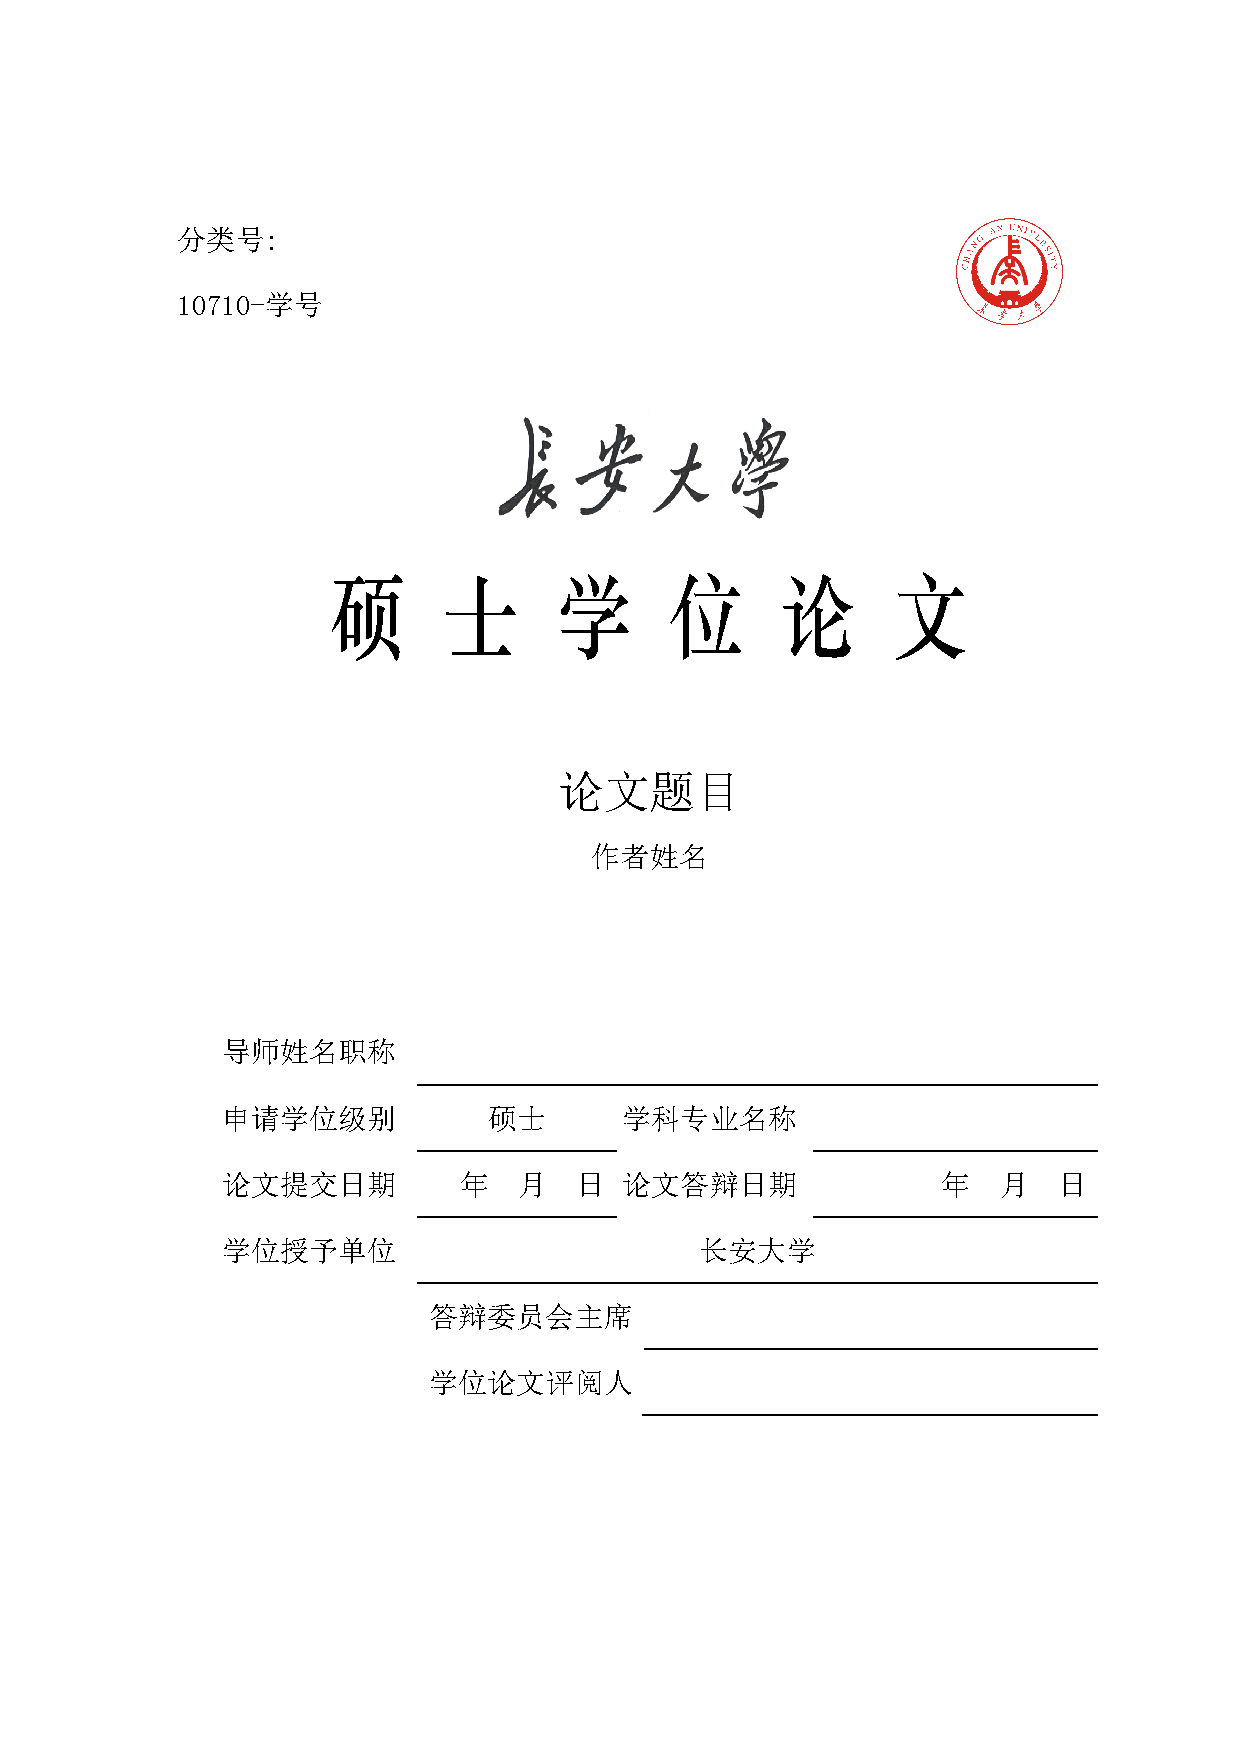
\includepdf[nup=1x1, delta=0mm 0mm,scale=1,pages={1-6}]{front/front.pdf}

\frontmatter
% 中英文摘要
% !TeX root = ../main.tex

\begin{abstract}
  为了提高研究生学位论文质量,统一学位论文的撰写和编辑的格式,便于信息的收集、存储、检索、利用和交流、传播。根据国家有关标准和学校实际,制定本规范。
  
学位论文的定义:学位论文是表明作者从事科学研究取得创造性的结果或有了新的见解,并以此为内容撰写而成、作为提出申请授予相应的学位时评审用的学术论文。

硕士学位论文,要求对所研究的课题有新见解或新成果,并在理论上或实践上对国民经济建设或本门学科发展具有一定的意义,表明作者在本门学科掌握坚实的基础理论和系统的专门知识,具有从事科学研究工作或独立担负专门技术工作的能力。

博士学位论文,要求对所研究的课题在科学上或专门技术上做出创造性成果,并在理论上或实践上对国民经济建设或本门学科发展具有较大的意义,表明作者在本门学科掌握坚实宽广的基础理论和系统深入的专门知识,具有独立从事科学研究工作的能力。

  本文的创新点主要有:
  \begin{itemize}
    \item 用例子来解释模板的使用方法;
    \item 用废话来填充无关紧要的部分;
    \item 一边学习摸索一边编写新代码。
  \end{itemize}

  关键词是为了文献标引工作、用以表示全文主要内容信息的单词或术语。
  关键词不超过 5 个,每个关键词中间用分号分隔。
  英文摘要的关键词与中文摘要的关键词应完全一致。

  \keywords{学位论文,\LaTeX{},模板}
\end{abstract}
\cleardoublepage
\begin{enabstract}
  An abstract of a dissertation is a summary and extraction of research work
  and contributions.
  Included in an abstract should be description of research topic and research
  objective, brief introduction to methodology and research process, and
  summarization of conclusion and contributions of the research.  An abstract
  should be characterized by independence and clarity and carry identical
  information with the dissertation.
  It should be such that the general idea and major contributions of the
  dissertation are conveyed without reading the dissertation.

  An abstract should be concise and to the point.
  It is a misunderstanding to make an abstract an outline of the dissertation
  and words ``the first chapter'', ``the second chapter'' and the like should
  be avoided in the abstract.

  Key words are terms used in a dissertation for indexing, reflecting core
  information of the dissertation.
  An abstract may contain a maximum of 5 key words, with semi-colons used in
  between to separate one another.

  \enkeywords{Dissertation, \LaTeX{}, template}
\end{enabstract}


\tableofcontents
% 图目录
\listoffigures
% 表目录
\listoftables
% 主要符号表
% !TeX root = ../main.tex

\begin{notation}

  \begin{center}
    \begin{tabular}{rl}
      $a$      & The number of angels per unit area     \\
      $N$      & The number of angels per needle point  \\
      $A$      & The area of the needle point           \\
      $\sigma$ & The total mass of angels per unit area \\
      $m$      & The mass of one angel                  \\
    \end{tabular}
  \end{center}

\end{notation}



% 也可以使用 nomencl 宏包

% \printnomenclature

% \nomenclature{$a$}{The number of angels per unit area}
% \nomenclature{$N$}{The number of angels per needle point}
% \nomenclature{$A$}{The area of the needle point}
% \nomenclature{$\sigma$}{The total mass of angels per unit area}
% \nomenclature{$m$}{The mass of one angel}



\mainmatter
% !TeX root = ../main.tex

\chapter{绪论}
\section{论文的基本要求}
论文应立论正确、推理严谨、说明透彻、数据可靠。

论文应结构合理、层次分明、叙述准确、文字简练、文图规范。对于涉及作者创新性工作和研究特点的内容应重点论述,做到数据或实例丰富、分析全面深入。文中引用的文献资料必须注明来源,使用的计量单位、绘图规范应符合国家标准。

论文的学术水平应满足规定的要求。

学位论文主体部分的篇幅(包含图、表和公式),硕士学位论文一般为40~60页,博士学位论文一般为60~100 页。提倡文笔简洁、用语规范。
\cite{Taylor2008Medical,Pham2000Current}。
\section{论文内容}
包括:选题的背景、依据及意义;文献及相关研究综述、研究及设计方案、试验方法、装置和试验结果;理论的证明、分析和结论;重要的计算、数据、图表、曲线及相关分析;必要的附录、相关的参考文献目录等。
对于合作完成的项目,论文的内容应侧重本人的研究工作。论文中有关与指导教师或他人共同研究、试验的部分以及引用他人研究成果的部分均要明确说明。

\subsection{二级节标题}

\subsubsection{三级节标题}
\paragraph{四级节标题}

\subparagraph{五级节标题}




\section{脚注}

Lorem ipsum dolor sit amet, consectetur adipiscing elit, sed do eiusmod tempor
incididunt ut labore et dolore magna aliqua.
\footnote{Ut enim ad minim veniam, quis nostrud exercitation ullamco laboris
nisi ut aliquip ex ea commodo consequat.
Duis aute irure dolor in reprehenderit in voluptate velit esse cillum dolore
eu fugiat nulla pariatur.}


% !TeX root = ../main.tex

\chapter{论文的主要结构及装订顺序}
学位论文一般应由11个部分组成,装订顺序依次为:

\begin{enumerate}
\item 封面(中、英文扉页)
\item 论文独创性声明和论文知识产权权属声明
\item 中文摘要
\item 英文摘要
\item 目录
\item 图表清单及主要符号表(根据具体情况可省略)
\item 主体部分(包括绪论、正文、结论等部分)
\item 参考文献
\item 附录
\item 攻读学位期间取得的研究成果
\item 致谢
\end{enumerate}


% !TeX root = ../main.tex

\chapter{论文格式规范}

\section{论文的文字及书写}

\subsection{论文的文字}

研究生学位论文一般用中文撰写,采用国家正式公布实施的简化汉字和法定的计量单位。也可以用英文撰写,但须同时提交用中文撰写的详细摘要。
\begin{enumerate}
  \item 来华留学生学位论文的目录、主体部分和致谢等可用英文撰写;但封面、独创性声明和权属声明应用中文撰写,硕士生须同时提交3000字左右的中文详细摘要,博士生须同时提交5000字左右的中文详细摘要。
  \item 外语专业的学位论文的目录、主体部分和致谢等应用所学专业相应的语言撰写;但封面、独创性声明和权属声明应用中文撰写,摘要应使用中文和所学专业相应的语言对照撰写。
\end{enumerate}

\subsection{论文的书写}

学位论文一律采用A4(70g)幅面白色纸张,封面、封底采用白色布纹纸张,中、英文扉页、独创性声明和使用授权书采用单面印刷,从中文摘要开始采用双面印刷。

\subsection{字体和字号}

\begin{itemize}
\item 章标题:三号黑体居中
\item 节标题:四号黑体居左
\item 条标题:小四号黑体居左
\item 主体部分:小四号宋体
\item 页码:五号宋体
\item 数字和字母: Times New Roman
\end{itemize}

\section{论文页面设置}

\subsection{页边距及行距}

学位论文的上边距:25mm;下边距:25mm;左边距:30mm;右边距:20mm。
章、节、条三级标题为单倍行距,段前、段后各设为0.5行(即前后各空0.5行)。
主体部分为1.5倍行距,段前、段后无空行(即空0行)。

\subsection{页眉}

页眉的上边距为15mm,页脚的下边距为15mm。页眉内容:页眉标注从论文主体部分开始(绪论或第一章),页眉用五号宋体,居中排列。奇偶页不同。奇数页页眉为章序及章标题,例如:“第四章  路基病害类型及分布规律”,偶数页页眉为“长安大学博士学位论文”或“长安大学硕士学位论文”。格式为页眉的文字内容之下划一条横线,线长与页面齐宽。

\subsection{页码}
论文页码从“主体部分”开始,直至“致谢”结束,用五号阿拉伯数字连续编码,页码位于页脚居中。

封面(中、英文扉页)、学位论文的独创性声明和权属声明不编入页码。

摘要、目录、图表清单、主要符号表用五号小罗马数字连续编码,页码位于页脚居中。

\section{名词术语}

科技名词术语及设备、元件的名称,应采用国家标准或部颁标准中规定的术语或名称。标准中未规定的术语要采用行业通用术语或名称。全文名词术语必须统一。特殊名词或新名词应在适当位置加以说明或注解。

采用英语缩写词时,除本行业广泛应用的通用缩写词外,文中第一次出现的缩写词应该用括号注明英文全称。

\section{物理量名称、符号与计量单位}

文中所用的物理量、符号与单位一律采用国家正式公布实施的《中华人民共和国法定计量单位》及国家标准《量和单位》(GB3100~3102)。

\section{图、表及其附注}

图和表应安排在主体部分中第1次提及该图、表的文字下方。当图或表不能安排在该页时,应安排在该页的下一页。

\subsection{图}

图包括曲线图、结构图、示意图、图解、框图、流程图、记录图、布置图、地图、照片、图版等。

图应具有“自明性”,即只看图、图题和图例,不阅读正文,就可理解图意。图的编号应采用阿拉伯数字分章依续编号,如:“图3.2”。

图题应明确简短,用五号宋体加粗,数字和字母为五号Times New Roman体加粗,图的编号与图题之间应空半角2格。图的编号与图题应置于图下方的居中位置。图内文字为5号宋体,数字和字母为5号Times New Roman体。曲线图的纵横坐标必须标注“量、标准规定符号、单位”,此三者只有在不必要标明(如无量刚等)的情况下方可省略。坐标上标注的量的符号和缩略词必须与正文中一致。

照片图要求主题和主要部分的轮廓鲜明,如用放大缩小的复制品,必须清晰,反差适中。照片上应有表示目的物尺寸的标度。

\subsection{表}

一律使用三线表,与文字齐宽,上下边线,线粗1.5 磅,表内线,线粗1 磅。例如表2-1;

表的编排,一般是内容和测试项目由左至右横读,数据依序竖读。表应有自明性。

表的编号应采用阿拉伯数字分章依续编号,如:“表2.5”。表题应明确简短,用五号宋体加粗,数字和字母为五号Times New Roman体加粗,表的编号与表题之间应空半角2格。表的编号与表题应置于表上方的居中位置。表内文字为5号宋体,数字和字母为5号Times New Roman体。

如某个表需要转页接排,在随后的各页上应重复表的编排。编号后跟表题(可省略)和“(续)”,如下所示:

表2.1  路基各边界热流密度(续)

续表应重复表头和关于单位的陈述。

\subsection{附注}

图、表中若有附注时,附注各项的序号一律用“附注 + 阿拉伯数字 + 冒号” ,如:“附注1:”。附注写在图、表的下方,一般采用5号宋体。

\section{公式}

文中公式的编号采用阿拉伯数字按章编排,用圆括号括起写在右边行末,其间不加虚线。如第一章第1个公式序号为“(1.1)”, 附录A中的第1个公式为“(A1)”等。文中引用公式时,一般用“见式(1.1)”或“由公式(1.1)”。

\section{注释}

学位论文中有个别名词或情况需要解释时,可加注说明,注释用页末注(将注文放在加注页的下端),而不用篇末注(将全部注文集中在文章末尾)和行中注(夹在论文主体部分中的注)。注号用阿拉伯数字上标标注,如:“注1”

\section{保密论文}

鼓励对学位论文进行去密处理,减少不必要的保密学位论文数量。去密处理时一般应去掉应用背景,与保密项目相关的技术指标和关键数据,使论文变成纯理论和技术的研究,达到可以在论文评审人员范围内公开或阅读的程度。对于技术和方法的保密,应该通过申请专利来保护,而不是把学位论文变为保密论文。

确实需要保密的论文由指导教师根据论文的情况提出并填写《长安大学涉密学位(毕业)论文定密审批表》,
校保密工作委员会按照国家规定的保密条例进行审批。
保密审批通过的论文需在封面直接把相应的“密级$\bigstar$  % TODO: 打五角星
”及“保密期限”标注在右上角,密级按由低到高可分为“秘密”、“机密”、“绝密”三级。

% !TeX root = ../main.tex

\chapter{浮动体的排版}
图和表应安排在主体部分中第1次提及该图、表的文字下方。
当图或表不能安排在该页时,应安排在该页的下一页。

\section{表格}

编制表格应简单明了,表达一致,明晰易懂,表文呼应、内容一致。
排版时表格字号略小,或变换字体,尽量不分页,尽量不跨节。
表格太大需要转页是,需要在续表上方注明“续表”,表头页应重复排出。

\subsection{三线表}

一律使用三线表,与文字齐宽,上下边线,线粗1.5 磅,表内线,线粗1 磅,
可直接使用\verb|\toprule|、\verb|\midrule|、\verb|\cmidrule{}|、\verb|\bottomrule|生成表格线,
如\autoref{tab:exampletable1},使用\verb|tabular*|环境指定表格宽度,
并利用\verb|@{\extracolsep{\fill}}|使内容自动伸展。
\begin{table}[htb]
  \centering
  \caption{三线表}
  \label{tab:exampletable1}
  \begin{tabular*}{0.6\linewidth}{c@{\extracolsep{\fill}}*{1}{c}}
    \toprule
    类型   & 描述                                       \\
    \midrule
    挂线表 & 挂线表也称系统表、组织表,用于表现系统结构 \\
    无线表 & 无线表一般用于设备配置单、技术参数列表等   \\
    卡线表 & 卡线表有完全表,不完全表和三线表三种       \\
    \bottomrule
  \end{tabular*}
\end{table}

\subsection{附注}
图、表中若有附注时,附注各项的序号一律用“附注 + 阿拉伯数字 + 冒号” ,如:“附注1:”。
附注写在图、表的下方,一般采用5号宋体。

针对撰写规范的规定,模板自定义了\verb|notetabular|环境创建带附注的表格,如\autoref{tab:exampletable2}。
使用方法与\verb|tabular*|类似,只是多了\verb|\tnote|参数。
\begin{table}
  \centering
  \caption{创建带附注表格}
  \label{tab:exampletable2}
  \begin{notetabular}{0.6\linewidth}{c@{\extracolsep{\fill}}*{2}{c}}  % 基本参数与tabular*一致
    {
      \tnote{竖向合并单元格,可能需要手动调整内容位置}
      \tnote[\hspace{2\ccwd}附注4]{自定义编号和缩进}
    }  % 附注内容须提前输入
    \toprule
    \multirow{2}{*}[-1.5mm]{Header 1\tmark} & \multicolumn{2}{c}{Header 2}\\
    \cmidrule{2-3}
    & Header 2.1& Header 2.2\\
    \midrule
    foo 1\tmark[4] & foo 2\tmark[4] & foo 3\\
    \bottomrule
  \end{notetabular}
\end{table}

\subsection{长表格}

如某个表需要转页接排,在随后的各页上应重复表的编排,
编号后跟表题(可省略)和“(续)”,
可以使用\pkg{longtable}宏包创建跨页表格。
续表应重复表头和关于单位的陈述。

\begin{longtable}{l@{\extracolsep{\fill}}*{1}{l}}
  \caption{\pkg{longtable}命令汇总\label{tab:exampletable3}} \\
  \toprule
  命令& 说明\\
  \midrule
  \endfirsthead
  \multicolumn{2}{l}{(续)}\\
  \toprule
  命令& 说明\\
  \midrule
  \endhead
  \bottomrule
  \endfoot
  \bottomrule
  \bottomrule[0pt]  % 添加间距
  \multicolumn{2}{l}{附注1:该命令产生的是页脚注,见\autoref{section:footnote};}\\
  \multicolumn{2}{l}{附注2:使用tmark(见\autoref{tab:exampletable2})配合endlatfoot创建长表格附注。}\\
  \endlastfoot
  不填写(默认)& 表格居中\\
  \verb|[c]|& 表格居中\\
  \verb|[l]|& 表格左对齐\\
  \verb|[r]|& 表格右对齐\\
  \verb|\\|& 结束一行表格\\
  \verb|\\[距离]|& 结束一行,并增加额外间距\\
  \multicolumn{2}{c}{(以下是为方便演示增加的额外间距)}\\[13cm]
  \verb|\\*|& 结束一行,并禁止在此分页\\*
  \verb|\kill|& 当前行不输出,只参与宽度计算\\
  xxxxxxxxxxxxxxxxxxxxxxxxxxxxxxxxxx&xxxxxxxxxxxxxxxxxxxxxxxxxxxxxxxxxxx\kill
  \verb|\endhead|& 此命令以上部分是每页的表头\\
  \verb|\endfirsthead|& 此命令以上部分是表格第一页的表头\\
  \verb|\endfoot|& 此命令以上部分是每页的表尾\\
  \verb|\endlastfoot|& 此命令以上部分是表格最后一页的表尾\\
  \verb|\caption{标题}|& 生成带编号的标题\\
  \verb|\caption*{标题}|& 生成不带编号的标题\\
  \verb|\newpage|& 强制分页\\
  \verb|\pagebreak[程度]|& 允许分页的程度(0-4)\\
  \verb|\nopagebreak[程度]|& 禁止分页的程度(0-4)\\
  \verb|\footnote|\tmark[1]& 使用脚注,注意不能用在表格头尾\\
  \verb|\footnotemark|& 单独产生脚注编号,不能用在表格头尾\\
  \verb|\footnotetext|& 单独产生脚注文字\\
  \verb|\LTleft|& 对齐方式留空时,表格左边的间距,默认为\verb|\fill|\\
  \verb|\LTright|& 对齐方式留空时,表格右边的间距,默认为\verb|\fill|\\
  \verb|\LTpre|& 表格上方间距,默认为\verb|\bigskipamount|\\
  \verb|\LTpost|& 表格下方间距,默认为\verb|\bigskipamount|\\
  \verb|\LTcapwidth|& 表格标题的宽度,默认为4\,in\\
\end{longtable}


\section{图}
图包括曲线图、结构图、示意图、图解、框图、流程图、记录图、布置图、地图、照片、图版等。
图应具有“自明性”,即只看图、图题和图例,不阅读正文,就可理解图意。
图的编号应采用阿拉伯数字分章依续编号,如:“\autoref{fig:epslogo}”。

\subsection{插入图片}
有的同学可能听说“\LaTeX{} 只能使用 eps 格式的图片”,甚至把 jpg 格式转为 eps。
事实上,这种做法已经过时。
而且每次编译时都要要调用外部工具解析 eps,导致降低编译速度。
所以我们推荐矢量图直接使用 pdf 格式,位图使用 jpeg 或 png 格式。
\begin{figure}[htb]
  \centering
  
\includegraphics[width=0.35\linewidth]{chdcolorlogo.eps}
  \caption{插入eps图片}
  \label{fig:epslogo}
  \note{附注1:现已不推荐使用。}
\end{figure}

\pkg{Texlive}中有许多自带的工具,比如可以利用\pkg{epstopdf}将eps图片转为pdf,
利用\pkg{pdfcrop}裁剪pdf图片,这些工具可在
\,\verb|Texlive|\verb|\版本|\verb|\bin|\verb|\win32|\,文件夹中找到,
或者直接通过命令行使用,本模板\pkg{figure}文件夹中的pdf即是通过\pkg{epstopdf}得到的。
\begin{figure}[htb]
  \centering
  
\includegraphics[width=0.35\linewidth]{chdcolorlogo.pdf}
  \caption{插入pdf图片}
  \label{fig:pdflogo}
\end{figure}

\subsection{并排放置图片}

关于图片的并排,推荐使用较新的 \pkg{subcaption} 宏包,
不建议使用 \pkg{subfigure} 或 \pkg{subfig} 等宏包。\footnote{此三个宏包不能同时导入}
以下为\pkg{subcaption} 宏包几种排列子图的方法。
\begin{figure}
  \centering
  \subcaptionbox{logo1\label{fig:logo1}}[.3\linewidth]{
\includegraphics[width=.7\linewidth]{chdredlogo.pdf}}
  \subcaptionbox{logo2\label{fig:logo2}}[.3\linewidth]{
\includegraphics[width=.7\linewidth]{chdredlogo.pdf}}
  \caption{使用\textsf{subcaptionbox}排列子图}
  \note{附注1:使用\textsf{subcaptionbox}时,\textsf{label应放在标题中}}
\end{figure}

\begin{figure}
  \centering
  \begin{subfigure}{.3\linewidth}
    \centering
    
\includegraphics[width=.7\linewidth]{chdbluelogo.pdf}
    \caption{logo1}
  \end{subfigure}
  \begin{subfigure}{.3\linewidth}
    \centering
    
\includegraphics[width=.7\linewidth]{chdbluelogo.pdf}
    \caption{logo2}
  \end{subfigure}
  \caption{使用\textsf{subfigure}排列子图}
\end{figure}

\begin{figure}
  \centering
  \begin{minipage}{.3\linewidth}
    \centering
    
\includegraphics[width=.7\linewidth]{chdblacklogo.pdf}
    \subcaption{logo1}
  \end{minipage}
  \centering
  \begin{minipage}{.3\linewidth}
    \centering
    
\includegraphics[width=.7\linewidth]{chdblacklogo.pdf}
    \subcaption{logo2}
  \end{minipage}
  \caption{使用使用\textsf{minipage}和\textsf{subcaption}排列子图}
\end{figure}

\subsection{跨页放置图片}

跨页放置子图,需要定义两个\pkg{figure}环境,并对\pkg{figure}的计数器进行修改,
好在\pkg{caption}提供了一个简化的操作,通过\verb|\ContinuedFloat|命令即可实现计数器的接续,
如\autoref{fig:cross}。
\begin{figure}[b]
  \centering
  \begin{subfigure}{\linewidth}
    \centering
    
\includegraphics[width=.4\linewidth]{chdblacklogo.pdf}
    \hspace{1cm}
    
\includegraphics[width=.4\linewidth]{chdblacklogo.pdf}
    \caption{blacklogo}
  \end{subfigure}
  \begin{subfigure}{\linewidth}
    \centering
    
\includegraphics[width=.4\linewidth]{chdbluelogo.pdf}
    \hspace{1cm}
    
\includegraphics[width=.4\linewidth]{chdbluelogo.pdf}
    \caption{bluelogo}
  \end{subfigure}
\end{figure}

\begin{figure}[t]
  \centering
  \ContinuedFloat
  \begin{subfigure}{\linewidth}
    \centering
    
\includegraphics[width=.4\linewidth]{chdredlogo.pdf}
    \hspace{1cm}
    
\includegraphics[width=.4\linewidth]{chdredlogo.pdf}
    \caption{redlogo}
  \end{subfigure}
  \begin{subfigure}{\linewidth}
    \centering
    
\includegraphics[width=.4\linewidth]{chdcolorlogo.pdf}
    \hspace{1cm}
    
\includegraphics[width=.4\linewidth]{chdcolorlogo.pdf}
    \caption{colorlogo}
  \end{subfigure}
  \caption{使用\textsf{ContinuedFloat}排版跨页图片\label{fig:cross}}
\end{figure}

\mbox{}
% !TeX root = ../main.tex

\chapter{数学}

\section{数字和单位}

宏包 \pkg{siunitx} 提供了更好的数字和单位支持:
\begin{itemize}
  \item \num{12345.67890}
  \item \num{1+-2i}
  \item \num{.3e45}
  \item \num{1.654 x 2.34 x 3.430}
  \item \si{kg.m.s^{-1}}
  \item \si{\micro\meter} $\si{\micro\meter}$
  \item \si{\ohm} $\si{\ohm}$
  \item \numlist{10;20}
  \item \numlist{10;20;30}
  \item \SIlist{0.13;0.67;0.80}{\milli\metre}
  \item \numrange{10}{20}
  \item \SIrange{10}{20}{\degreeCelsius}
\end{itemize}



\section{数学符号和公式}

\LaTeX{} 默认按照美国的习惯排版数学公式和符号,
但是《撰写手册》要求数学符号依据《GB 3102.11--1993》执行,
与 \LaTeX{} 的习惯有所差异。
本模板基于 \pkg{unicode-math} 配置数学符号,以遵循国标的规定。

注意,\pkg{unicode-math} 宏包与 \pkg{amsfonts}, \pkg{amssymb}, \pkg{bm},
\pkg{mathrsfs}, \pkg{upgreek} 等宏包\emph{不}兼容。
本模板作了处理,用户可以直接使用这些宏包的命令,如 \cs{bm}, \cs{mathscr},
\cs{upGamma}。

本模板中数学符号的用法与 \LaTeX{} 传统有些区别:
\begin{itemize}
  \item 数学常数和特殊函数使用正体,
    如圆周率 $\symup{\pi}$、$\symup{\Gamma}$ 函数。
    应使用 \pkg{unicode-math} 宏包提供的 \cs{symup} 命令转为正体,
    如 \verb|\symup{\pi}|。
  \item 向量和矩阵粗斜体,应使用 \cs{symbf} 命令,
    如 \verb|\symbf{u}|、\verb|\symbf{A}|。
  \item 有限增量符号 $\increment$ (U+2206)应使用 \cs{increment} 命令。
  \item 微分符号 $\dif$ 使用正体,本模板提供了 \cs{dif} 命令。
\end{itemize}

除此之外,模板还提供了一些命令方便使用:
\begin{itemize}
  \item 常数 $\upe$:\verb|\upe|
  \item 负数单位 $\upi$:\verb|\upi|
  \item 圆周率 $\uppi$:\verb|\uppi|
  \item $\argmax$:\verb|\argmax|
  \item $\argmin$:\verb|\argmin|
\end{itemize}

关于数学符号更多的用法,参见 \pkg{unicode-math} 宏包的使用说明和符号列表
\pkg{unimath-symbols}。

在编辑数学公式时,最好避免直接使用字体命令,
而应该定义一些语义命令取代字体命令,
这样输入更简单,也让 \LaTeX{} 代码更有可读性,
而且还方便根据需要统一修改改格式,比如:
\begin{itemize}
  \item 向量 $\vec{x}$:\verb|\renewcommand\vec{\symbf}|
  \item 矩阵 $\mat{A}$:\verb|\newcommand\mat{\symbf}|
  \item 张量 $\ts{T}$: \verb|\newcommand\ts{\symbfsf}|
\end{itemize}

更多的例子:
\begin{equation}
  \upe^{\upi\uppi} + 1 = 0
\end{equation}
\begin{equation}
  \frac{\dif^2 u}{\dif t^2} = \int f(x) \dif x
\end{equation}
\begin{equation}
  \argmin_x f(x)
\end{equation}
\begin{equation}
  \mat{A} \vec{x} = \lambda \vec{x}
\end{equation}



\section{定理和证明}

示例文件中使用 \pkg{amsthm} 宏包配置了定理、引理和证明等环境。
用户也可以使用  \pkg{ntheorem} 宏包。

\begin{definition}
  If the integral of function $f$ is measurable and non-negative, we define
  its (extended) \textbf{Lebesgue integral} by
  \begin{equation}
    \int f = \sup_g \int g,
  \end{equation}
  where the supremum is taken over all measurable functions $g$ such that
  $0 \le g \le f$, and where $g$ is bounded and supported on a set of
  finite measure.
\end{definition}

\begin{example}
  Simple examples of functions on $\real^d$ that are integrable
  (or non-integrable) are given by
  \begin{equation}
    f_a(x) =
    \begin{cases}
      |x|^{-a} & \text{if } |x| \le 1, \\
      0        & \text{if } x > 1.
    \end{cases}
  \end{equation}
  \begin{equation}
    F_a(x) = \frac{1}{1 + |x|^a}, \qquad \text{all } x \in \real^d.
  \end{equation}
  Then $f_a$ is integrable exactly when $a < d$, while $F_a$ is integrable
  exactly when $a > d$.
\end{example}

\begin{lemma}[Fatou]
  Suppose $\{f_n\}$ is a sequence of measurable functions with $f_n \geq 0$.
  If $\lim_{n \to \infty} f_n(x) = f(x)$ for a.e. $x$, then
  \begin{equation}
    \int f \le \liminf_{n \to \infty} \int f_n.
  \end{equation}
\end{lemma}

\begin{remark}
  We do not exclude the cases $\int f = \infty$,
  or $\liminf_{n \to \infty} f_n = \infty$.
\end{remark}

\begin{corollary}
  Suppose $f$ is a non-negative measurable function, and $\{f_n\}$ a sequence
  of non-negative measurable functions with
  $f_n(x) \le f(x)$ and $f_n(x) \to f(x)$ for almost every $x$. Then
  \begin{equation}
    \lim_{n \to \infty} \int f_n = \int f.
  \end{equation}
\end{corollary}

\begin{proposition}
  Suppose $f$ is integrable on $\real^d$. Then for every $\epsilon > 0$:
  \begin{enumerate}
    \renewcommand{\theenumi}{\roman{enumi}}
    \item There exists a set of finite measure $B$ (a ball, for example) such
      that
      \begin{equation}
        \int_{B^c} |f| < \epsilon.
      \end{equation}
    \item There is a $\delta > 0$ such that
      \begin{equation}
        \int_E |f| < \epsilon \qquad \text{whenever } m(E) < \delta.
      \end{equation}
  \end{enumerate}
\end{proposition}

\begin{theorem}
  Suppose $\{f_n\}$ is a sequence of measurable functions such that
  $f_n(x) \to f(x)$ a.e. $x$, as $n$ tends to infinity.
  If $|f_n(x)| \le g(x)$, where $g$ is integrable, then
  \begin{equation}
    \int |f_n - f| \to 0 \qquad \text{as } n \to \infty,
  \end{equation}
  and consequently
  \begin{equation}
    \int f_n \to \int f \qquad \text{as } n \to \infty.
  \end{equation}
\end{theorem}

\begin{proof}
  Trivial.
\end{proof}

\newtheorem*{axiomofchoice}{Axiom of choice}
\begin{axiomofchoice}
  Suppose $E$ is a set and ${E_\alpha}$ is a collection of
  non-empty subsets of $E$. Then there is a function $\alpha
  \mapsto x_\alpha$ (a ``choice function'') such that
  \begin{equation}
    x_\alpha \in E_\alpha,\qquad \text{for all }\alpha.
  \end{equation}
\end{axiomofchoice}

\newtheorem{observation}{Observation}
\begin{observation}
  Suppose a partially ordered set $P$ has the property
  that every chain has an upper bound in $P$. Then the
  set $P$ contains at least one maximal element.
\end{observation}
\begin{proof}[A concise proof]
  Obvious.
\end{proof}

\section{算法}
\begin{algorithm}[H]
\SetAlgoLined
\KwData{this text}
\KwResult{how to write algorithm with \LaTeX2e }
initialization\;
\While{not at end of this document}{
read current\;
\eIf{understand}{
go to next section\;
current section becomes this one\;
}{
go back to the beginning of current section\;
}
}
\caption{How to write algorithms}
\end{algorithm}

% !TeX root = ../main.tex

\chapter{引用文献的标注}

模板使用 \pkg{natbib} 宏包来设置参考文献引用的格式,
更多引用方法可以参考该宏包的使用说明。



\section{顺序编码制}

\subsection{角标数字标注法}

\citestyle{super}
\noindent
\begin{tabular}{l@{\quad$\Rightarrow$\quad}l}
  \verb|\cite{knuth86a}|         & \cite{knuth86a}         \\
  \verb|\citet{knuth86a}|        & \citet{knuth86a}        \\
  \verb|\cite[42]{knuth86a}|     & \cite[42]{knuth86a}     \\
  \verb|\cite{knuth86a,tlc2}|    & \cite{knuth86a,tlc2}    \\
  \verb|\cite{knuth86a,knuth84}| & \cite{knuth86a,knuth84} \\
\end{tabular}


\subsection{数字标注法}

\citestyle{numbers}
\noindent
\begin{tabular}{l@{\quad$\Rightarrow$\quad}l}
  \verb|\cite{knuth86a}|         & \cite{knuth86a}         \\
  \verb|\citet{knuth86a}|        & \citet{knuth86a}        \\
  \verb|\cite[42]{knuth86a}|     & \cite[42]{knuth86a}     \\
  \verb|\cite{knuth86a,tlc2}|    & \cite{knuth86a,tlc2}    \\
  \verb|\cite{knuth86a,knuth84}| & \cite{knuth86a,knuth84} \\
\end{tabular}



\section{著者-出版年制标注法}

\citestyle{authoryear}
\noindent
\begin{tabular}{l@{\quad$\Rightarrow$\quad}l}
  \verb|\cite{knuth86a}|         & \cite{knuth86a}         \\
  \verb|\citep{knuth86a}|        & \citep{knuth86a}        \\
  \verb|\cite[42]{knuth86a}|     & \cite[42]{knuth86a}     \\
  \verb|\cite{knuth86a,tlc2}|    & \cite{knuth86a,tlc2}    \\
  \verb|\cite{knuth86a,knuth84}| & \cite{knuth86a,knuth84} \\
\end{tabular}

\vskip 2ex \citestyle{super}
注意,参考文献列表中的每条文献在正文中都要被引用
\cite{slg,lyc,ljs,cgw,cjb,kqy,yhs,yx,dwx,jxz,wjk,syw,wf,xd,twh,huston}。

% !TeX root = ../main.tex

\begin{summary}[结论与展望]  % 此处[]内缺省为“结论"
    学位论文的结论单独作为一章,但不加章号。
    
    该模板创建了一个符合要求的结论环境。
    \section*{结论}
    通过研究得到以下结论:
    \section*{展望}
    虽然得到了一些有价值的结论,但由于篇幅和资料限制,仍有许多问题可以作进一步研究:
\end{summary}
\bibliography{bibs/refs} % 参考文献

% 附录
\appendix
\chapter{论文规范}

\backmatter
% !TeX root = ../main.tex

\begin{publications}

\section*{已发表论文}

\begin{enumerate}
\item A A A A A A A A A
\item A A A A A A A A A
\item A A A A A A A A A
\end{enumerate}

\section*{待发表论文}

\begin{enumerate}
\item A A A A A A A A A
\item A A A A A A A A A
\item A A A A A A A A A
\end{enumerate}

\section*{研究报告}
\begin{enumerate}
\item A A A A A A A A A
\item A A A A A A A A A
\item A A A A A A A A A
\end{enumerate}

\end{publications}

% !TeX root = ../main.tex

\begin{acknowledgements}

在研究学习期间,我有幸得到了三位老师的教导,
他们是:我的导师,中国科大XXX研究员,中科院X昆明动物所马老师以及美国犹他大学的XXX老师。
三位深厚的学术功底,严谨的工作态度和敏锐的科学洞察力使我受益良多。
衷心感谢他们多年来给予我的悉心教导和热情帮助。

感谢XXX老师在实验方面的指导以及教授的帮助。
科大的XXX同学和XXX同学参与了部分试验工作,在此深表谢意。

\end{acknowledgements}


\end{document}
